\section{Applikation}                                   
I følgende afsnit gøres der rede for beslutningerne i forhold til udviklingen af applikationen.

\subsection{Styresystem}
Der findes forskellige styresystemer til mobiltelefoner i dag. De to mest brugte\cite{OS} er dog iOS \cite{iOS} og Android. \cite{Android} \\
IOS er Apples eget styresystem, som er udviklet i forhold til deres mobile og tablet enheder. \\
Android er et stort open source project, som bliver brugt på ca. 80\% af alle mobile og tablet enheder i dag. Der findes forskellige versioner af Android styresystemet alt efter, hvilken producent der har leveret enheder\cite{OS}. \\
Nogle af de kendte Android enheder leverendører er firmaer som Samsung, Huawei og HTC. De har alle en Android Core i deres styresystemer og har også alle videreudviklet styresystemet, så det passer specifikt til deres enheder.

Rambøll ønskede en applikation udviklet til iOS. Til en workshop med Rambøll fandt vi ud af, at der også var ansatte, som bruger Android. Derfor blev der aftalt at udvikle cross-platform.

\subsection{Cross-platform udviklingsværktøjer}
I denne sektion vil der være en kort beskrivelse af nogle udviklingsværktøjer til cross-platform.

\subsubsection{Xamarin}
Xamarin\cite{Xarmain} tilbyder en cross-platform, hvor der udvikles i C\#\cite{CSharp} og XAML\cite{XAML}.
Features Xamarin tilbyder:
\begin{itemize}[-]
	\item Integreret i Visual Studio.
	\item Fuld API Access til både iOS og Android.
	\item Deling af kode.
\end{itemize}

\subsubsection{PhoneGap}
PhoneGap\cite{PhoneGap} er en platform udviklet af Adobe\cite{Adobe}. Her bruges teknologier som HTML5\cite{HTML5}, JavaScripts\cite{JavaScript} og CSS\cite{CSS}. \\
Deres platform tilbyder nogle bonus features som:
\begin{itemize}[-]
	\item Build server.
	\item Easy share af applikationen.
	\item Mulitple plug-ins.
\end{itemize}

\clearpage

\subsubsection{Corona}
Corona\cite{Corona} tilbyder en cross-platform, hvor der udvikles i Lua scripting \cite{Lua}.
\begin{itemize}[-]
	\item Real time simulering.
	\item Live testing.
	\item Mange plug-in muligheder.
\end{itemize}

\subsection{Valg af cross-platform udviklingsværktøj}
I følgende afsnit redegøres for de beslutninger, der er taget angående valg af Xamarin.

Der var et lille kendskab til Xamarin fra et tidligere projekt lavet på Ingeniørhøjskolen Aarhus Universitet. \\
Xamarin giver mulighed for at skrive i C\#, som er et sprog, der er blevet undervist i på Ingeniørhøjskolen Aarhus Universitet, som er et højniveau sprog. \\
Xamarin blev i februar 2016 opkøbt af Microsoft, hvilket har betydet, at det siden da har været en integreret del af Microsoft Visual Studio, som er det fortrukne udviklingsværktøj.\\
Udvikler dokumentationen for Xamarin er også et plus. Hvis man sidder med et problem, har Xamarin lavet en meget grundig dokumentation, hvor man kan finde eksempler og guides, til hvordan forskellige dele i en applikaiton skal programmeres.

\subsection{Xamarin}
Denne sektion vil indeholde en mere dybdegående beskrivelse af, hvordan Xamarin platformen er bygget op.

Xamarin tilbyder en version der hedder Xamarin Forms\cite{Forms}. Fordelene ved at skrive i Xamarin Forms er, at man kan dele C\# kode for de forskellige applikationer.
På billedet herunder kan man se, hvordan User Interface koden og App Logic koden er delt på tværs af alle tre enheder. Der skal altså kun skrive sin App Logic og User Interface én gang, og så virker det på både iOS, Android og Windows.
\begin{figure}[H]
	\centering
	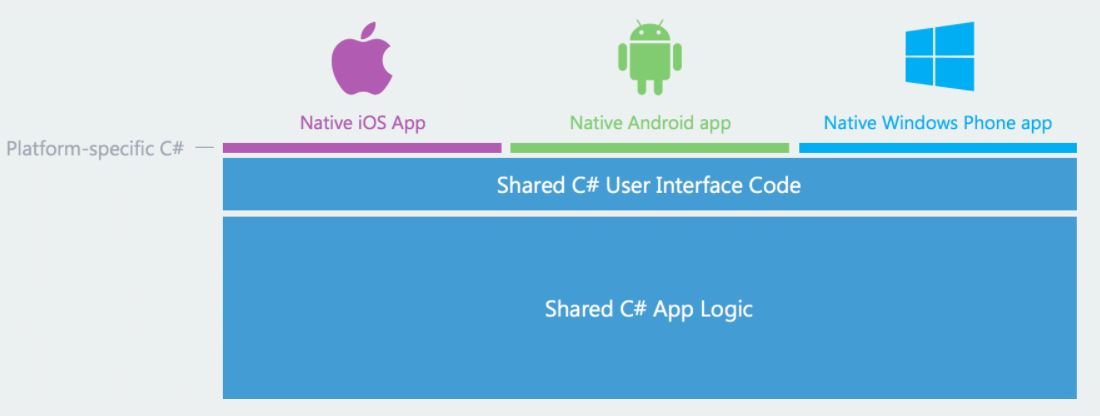
\includegraphics[width=1\linewidth]{Applikation/XarmarinShare.JPG}
	\caption{Kode deling i Xamarin Forms.\cite{Xarmain}}
	\label{fig:CodeShare}
\end{figure}

\clearpage

Xamarin kommer både med Xamarin.iOS og Xamarin.Android. Hvad dette gør er, at når koden kompiles, komplier den ned til native kode. IOS delen vil blive kompileret til ARM assembly, så ens app er native binære platform. Android kompileres, så den kører native Android APK. Så man vil får kompileret koden så den passer til den specifike enhed, man vil bruge. \\
Xamarin er baseret på C\# og ved hjælp af Xamarin.iOS og Xamarin.Android er det muligt, at kalde og binde det sammen med den eksisterende kode i både iOS og Android, via Xamarins automatiske binding generator. \\
Der bliver i både Xamarin.iOS og Xamarin.Android givet muligheder for at forbinde til alle API'er, der er nødvendige. \\

\begin{figure}[H]
	\centering
	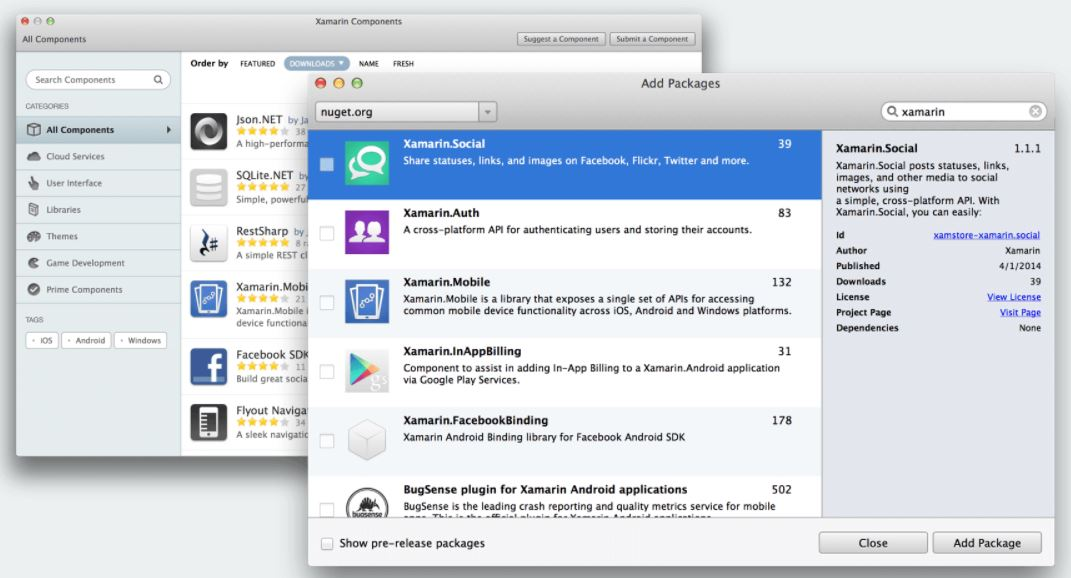
\includegraphics[width=0.7\linewidth]{Applikation/NuGet.JPG}
	\caption{NuGet og Xamarin Componet Store.\cite{Xarmain}}
	\label{fig:NuGet}
\end{figure}
Xamarin tilbyder også en masse ekstra komponenter, som kan integreres i applikationen. Det kan være alt fra web API'er til sikkerheds elementer.

\clearpage